\documentclass{article}

\usepackage{graphicx}
\usepackage{tikz}
\usepackage{tikzsymbols}
\usetikzlibrary{calc,patterns,shapes.geometric}
\pagestyle{empty}
\usepackage[margin=0pt]{geometry}
\geometry{papersize={14in,12in}}

\def\centerarc[#1](#2)(#3:#4:#5){\draw[#1] ($(#2)+({#5*cos(#3)},{#5*sin(#3)})$) arc (#3:#4:#5);}

\begin{document}
	\begin{figure}
		\centering
		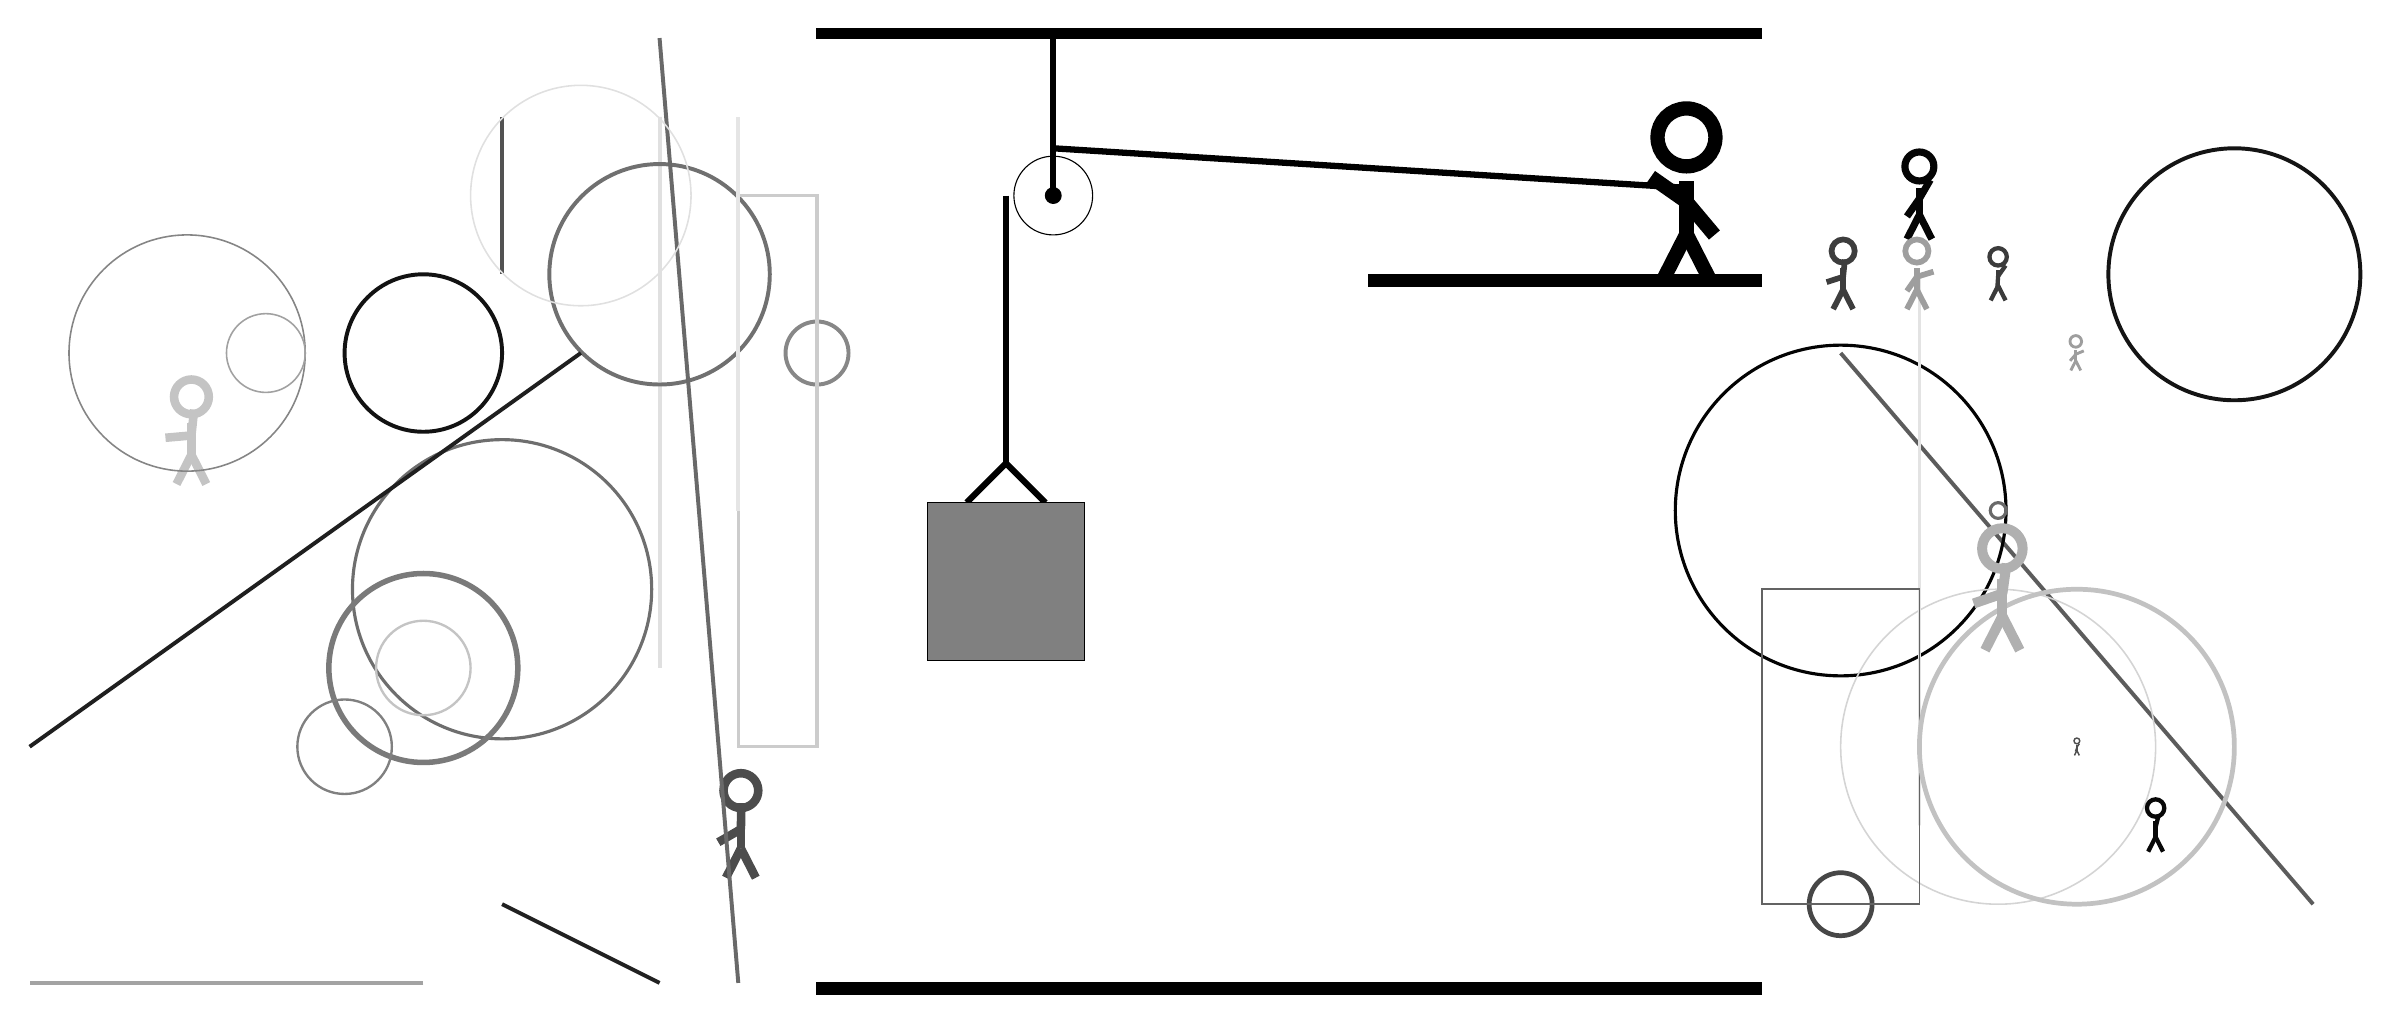
\begin{tikzpicture}
			%%%%% START %%%%%
			
			\draw[fill=black] (-2, 9) rectangle (10, 9.125);
			
			\draw (1, 7) circle (0.5);
			\draw[fill=black] (1, 7) circle (0.1);
			\draw[line width=0.8mm] (1, 9) -- (1, 7);
			
			\draw[line width=0.8mm](-0.1, 3.1) --  (0.4, 3.6) -- (0.9, 3.1);
			\draw[fill=black!50] (-0.6, 3.1) rectangle (1.4, 1.1);
			
			\draw[line width=0.8mm](0.4, 7) -- (0.4, 3.6);
			\centerarc[line width=0.8mm](1, 7)(90:180:0.6)
			\draw[line width=0.8mm](1, 7.6) -- (9, 7.1);
			
			\node at (9, 7) {\Strichmaxerl[10][-35][-50]};
			\draw[fill=black] (5, 6) rectangle (10, 5.85);
			
			\draw [line width=0.4mm, color=black!57](-6, 2) circle (1.9);
			
			\node[line width=0.3mm, color=black!98] at (12, 7) {\Strichmaxerl[5][55][60]};
			\node[line width=0.3mm, color=black!23] at (-10, 4) {\Strichmaxerl[6][5][84]};
			\draw[line width=0.5mm, color=black!68](-6, 8) -- (-6, 6);
			\node[line width=0.3mm, color=black!70] at (-3, -1) {\Strichmaxerl[6][30][89]};
			\draw[line width=0.5mm, color=black!64](11, 5) -- (17, -2);
			
			\draw[line width=0.5mm, color=black!36](-7, -3) -- (-12, -3);
			\draw [line width=0.7mm, color=black!52](-7, 1) circle (1.2);
			\draw [line width=0.6mm, color=black!72](11, -2) circle (0.4);
			\draw [line width=0.4mm, color=black!99](11, 3) circle (2.1);
			\draw [line width=0.5mm, color=black!47](-2, 5) circle (0.4);
			
			\node[line width=0.6mm, color=black!77] at (13, 6) {\Strichmaxerl[3][86][55]};
			\node[line width=0.6mm, color=black!38] at (14, 5) {\Strichmaxerl[2][49][23]};
			
			\draw [line width=0.2mm, color=black!17](13, 0) circle (2.0);
			\draw[line width=0.5mm, color=black!12] (-4, 8) rectangle (-4, 1);
			\draw [line width=0.5mm, color=black!56](-4, 6) circle (1.4);
			\draw[line width=0.5mm, color=black!87](-4, -3) -- (-6, -2);
			\draw[line width=0.4mm, color=black!11] (12, 6) rectangle (12, -1);
			\draw[line width=0.5mm, color=black!59](-3, -3) -- (-4, 9);
			\node[line width=0.7mm, color=black!38] at (12, 6) {\Strichmaxerl[4][55][17]};
			\draw [line width=0.3mm, color=black!23](-7, 1) circle (0.6);
			
			\node[line width=0.6mm, color=black!97] at (15, -1) {\Strichmaxerl[3][89][76]};
			
			\draw[line width=0.5mm, color=black!88](-5, 5) -- (-12, 0);
			\draw[line width=0.4mm, color=black!20] (-2, 0) rectangle (-3, 7);
			\draw [line width=0.5mm, color=black!93](-7, 5) circle (1.0);
			
			\draw[line width=0.5mm, color=black!10](-3, 3) -- (-3, 8);
			
			\draw [line width=0.2mm, color=black!48](-10, 5) circle (1.5);
			\draw [line width=0.4mm, color=black!59](13, 3) circle (0.1);
			\node[line width=0.5mm, color=black!69] at (14, 0) {\Strichmaxerl[1][70][56]};
			\draw[line width=0.2mm, color=black!61] (10, 2) rectangle (12, -2);
			\draw [line width=0.5mm, color=black!92](16, 6) circle (1.6);
			
			\draw [line width=0.6mm, color=black!24](14, 0) circle (2.0);
			\draw [line width=0.3mm, color=black!50](-8, 0) circle (0.6);
			
			\draw [line width=0.2mm, color=black!12](-5, 7) circle (1.4);
			\draw [line width=0.2mm, color=black!37](-9, 5) circle (0.5);
			\node[line width=0.6mm, color=black!76] at (11, 6) {\Strichmaxerl[4][18][84]};
			
			\node[line width=0.6mm, color=black!31] at (13, 2) {\Strichmaxerl[7][19][82]};
			
			\draw[fill=black] (-2, -3) rectangle (10, -3.15);
			
			%%%%% END %%%%%
		\end{tikzpicture}
	\end{figure}	
\end{document}